\documentclass[10pt,letterpaper]{article}
\usepackage[top=1in,bottom=1in,left=1in,right=1in]{geometry}
\usepackage{datetime}
\usepackage{natbib}      % http://merkel.zoneo.net/Latex/natbib.php
\usepackage{palatino}
\usepackage{verbatim}
\usepackage[normalem]{ulem}
\bibpunct{(}{)}{;}{a}{,}{,}

\usepackage{array}

\usepackage{chngpage}
\usepackage{stmaryrd}
\usepackage{amssymb}
\usepackage{amsmath}
\usepackage{graphicx}
\usepackage{lscape}
\usepackage{subfigure}
\usepackage[usenames,dvipsnames]{color}
\definecolor{myblue}{rgb}{0,0.1,0.6}
\definecolor{mygreen}{rgb}{0,0.3,0.1}
\usepackage[colorlinks=true,linkcolor=black,citecolor=mygreen,urlcolor=myblue]{hyperref}

\newcommand{\bocomment}[1]{\textcolor{Bittersweet}{BO says: #1}}

\newcommand{\ignore}[1]{}
\newcommand{\transpose}{^\mathsf{T}}
\newcommand{\inner}[1]{\langle #1 \rangle} 
\newcommand{\smallsec}[1]{\noindent \textbf{#1\ }}
\newcommand{\cmd}[1] {{\color{blue}\texttt{#1}}}
\newcommand{\todo}[1]{{\color{red} [TODO: #1]}}

\newcommand{\solution}[1]{{\color{myblue} \emph{[Solution:} 

#1 

\emph{End solution]}}}
\newcommand{\solutionnote}[1]{{\color{myblue} \emph{[Note:}

#1 

\emph{End note]}}}
\newcommand{\points}[1]{{\color{mygreen}\emph{[#1]\ \ }}}

\newcommand{\aone}{\diamondsuit}
\newcommand{\atwo}{\heartsuit}
\newcommand{\bone}{\triangle}
\newcommand{\btwo}{\Box}
\newcommand{\myand}{\ \land\ }
\newcommand{\myor}{\ \lor\ }
\newcommand{\mynot}{\lnot}

\title{
	Mini-project 6\\
	\Large{COMPSCI 370, Spring 2021, UMass Amherst} \\
	\Large{Instructor: Subhransu Maji} \\
	\Large{TAs: Chenyun Wu, Jong-Chyi Su}
}


\settimeformat{ampmtime}
\date{}

\begin{document}
	
\maketitle

\renewcommand\thesubsection{\thesection.\alph{subsection}}
\section*{Guidelines}
\paragraph{Submission.} Submit a \emph{single pdf} file via
Gradescope that includes your solutions, figures, and code. The latex
source file for the homework is provided in case you want to modify it
to produce your report. However, you are welcome to use other
typesetting software as long as the final output is a pdf.
For readability you may attach the code printouts at the end of the
solutions within the same pdf.
Similarly figures enable easy comparision of various approaches.
Poorly written or formatted reports will make it harder for us to
evaluate it and may lead to a deduction of credit.


\paragraph{Late policy.}
\begin{itemize}
\item You can use 7 late days, with up to 3 late days per assignment.
\item Once you have used all 7 late days, penalty is 25\% for each additional late day.
\item We will use your latest submission for grading and for calculating your late day usage.
\item There is no bonus if you don't use late days at all.
\end{itemize}


\paragraph{Plagiarism.}
We expect the students not to copy, refer to, or look at the solutions
in preparing their answers. We expect students to want to learn and
not google for answers. See the Universities' guidelines on academic
honesty (\url{https://www.umass.edu/honesty}).
Finally, we also ask you to not post the solutions online as the
problem sets might be used in future.


\paragraph{Collaboration.} The homework must be done individually,
except where otherwise noted in the assignments. 'Individually' means
each student must hand in their own answers, and each student must
write their own code in the programming part of the assignment. It is
acceptable, however, for students to collaborate in figuring out
answers and helping each other solve the problems, for example within
a study group.
We will be assuming that you will be taking the responsibility to make
sure you personally understand the solution to any work arising from
such a collaboration.


\paragraph{Python requirements.}
Our code is tested on Python 3.
The Python code depends on external
packages such as \cmd{scipy}, \cmd{numpy}, and \cmd{scikit-image}.
Take a look at the resources posted on the course page to set up the
appropriate programming environment and tutorial on basic concepts.


\paragraph{Using other programming languages.}
While we have made the starter code available in Python, 
feel free to implement the homework from scratch using your favorite
programming language. For example you are welcome to use Matlab, C, Java,
Octave or Julia, with the caveat that we may be able help you with
debugging.









\newpage

\section*{The MNIST dataset}
In this homework you will train classifiers to predict whether an
image is a ``$5$" or an ``$9$".

The file $\cmd{data.pkl}$ contains the dataset for this mini-project
which is a subset of the MNIST dataset~\footnote{\url{http://yann.lecun.com/exdb/mnist/}}.
You can load the dataset by $\cmd{data = pickle.load(open('data.pkl','rb'))}$. The data is split into $\cmd{train}$
and $\cmd{test}$ sets.


For each split, the features and labels are $\cmd{x}$ and $\cmd{y}$
respectively. E.g., $\cmd{data["train"]["x"]}$ is an array of size $28
\times 28 \times200$ containing $200$ digits.
The first 100 digits are ${5}$s and the remaining 100 digits are ${9}$s, each of size
$28 \times 28$.
Class labels are given by $\cmd{data["train"]["y"]}$. Thus, pixel
\cmd{(i,j)} in the the \cmd{k'th} training example is
\cmd{data["train"]["x"][i, j, k]} with label
\cmd{data["train"]["y"][k]}. The $\cmd{test}$ set contains $100$
examples from the two classes in the same format.


The features are simply binary pixel values, i.e., each pixel is
either 0 or 1. You can visualize the dataset using
$\cmd{montageDigits(x)}$ function. Below is the output of
$\cmd{montageDigits(data["train"]["x"])}$.

\begin{figure}[h]
\centering
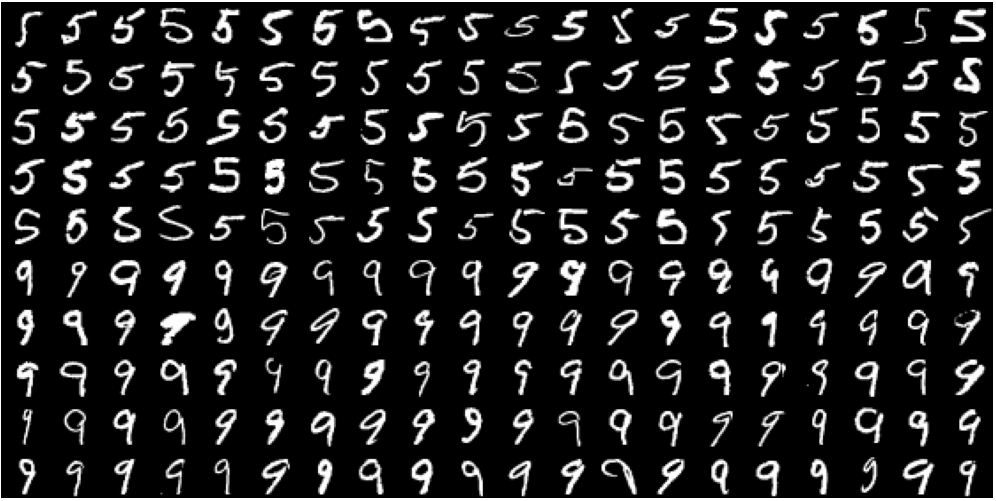
\includegraphics[width=0.85\linewidth]{montage59.png}
\end{figure}

The function \cmd{avgImg = montageDigits(x)} additionally returns the average of all images in x. You can visualize it using \cmd{plt.imshow(scores, cmap="gray")}. This is useful for debugging your feature selection algorithms in decision trees. Below are the outputs of: 
\begin{itemize}
\item \cmd{avgImg = montageDigits(data["train"]["x"])}, i.e., all training images
\item \cmd{avgImg = montageDigits(data["train"]["x"][:, :, :100])},
  i.e., the first 100 digits, which are only the 5s. 
\item \cmd{avgImg = montageDigits(data["train"]["x"][:, :, 100:])},
  i.e., only the 9s. 
\end{itemize}

\begin{figure}[h]
\centering
\begin{tabular}{ccc}

\includegraphics[width=0.2\linewidth]{avg59.png} &

\includegraphics[width=0.2\linewidth]{avg5.png} &

\includegraphics[width=0.2\linewidth]{avg9.png} \\
all & 5s & 9s
\end{tabular}
\end{figure}

\newpage
\section{Decision trees [50 points]}

Answer the following questions of using decision trees for classification.
\begin{enumerate}
\item \cmd{(5 points)} What is the accuracy of an empty decision tree
  on the training set? Accuracy is the fraction of the examples
  correctly classified. What is the accuracy on the test set? Briefly explain your answer.

\item Suppose you are allowed to find the value of one pixel for
  predicting the label of the image. Which pixel should it be? This
  corresponds to a decision tree of depth 1.
  

\begin{enumerate}
\item \cmd{(15 points)} Implement \cmd{scoreFeatures(x, y)} in
  \cmd{decisionTrees.py}. The function returns a matrix of size
  $28\times 28$ that corresponds to the number of examples \cmd{x}
  that can be correctly classified if the value of that pixel was
  known.
Using this find the pixel that has the highest score. 
Include the code, the scores visualized as an image using \cmd{plt.imshow(scores, cmap="gray")}, 
and also write down the (i, j) coordinates of the pixel with the
highest score and the value of the score.

\item \cmd{(5 points)} Write down the decision tree that obtains the
  best classification in the form of an if-then-else statement. For
  example, "if pixel(5,10) == 1 then predict 5, else predict 9". The
  exact syntax is not important.
 
\item \cmd{(5 points)} Apply this rule on the test set. What accuracy does this rule obtain?
\end{enumerate}

\item Construct a decision tree of depth 2 to classify the data using
  the greedy learning algorithm.
Suppose (x,y) was the pixel selected in the previous step.
This divides the training data into two subsets, one for which
pixel(x,y) = 1, and another for which pixel(x,y) = 0.
The best pixel in the next level of the tree can be obtained by
repeating the previous step for each subset of the data.
\begin{enumerate}
\item \cmd{(15 points)} Apply the above to construct the next level of
  the tree. Write down the resulting classifier using if-then-else
  statements. For example,
\begin{verbatim}
if pixel(5,10) == 1
    if pixel(14,22) == 1
        predict 5;
    else
        predict 9;
    end
else 
    if pixel(11,6) == 1
        predict 5;
    else
        predict 9;
    end
end
\end{verbatim}
\item \cmd{(5 points)} Apply this rule on the test set. What accuracy does this rule obtain?
\end{enumerate}
\end{enumerate}


\section{K-nearest neighbor classifier [20 points]}
In this section, you will implement a k-nearest neighbor classifier in $\cmd{kNearestNeighbor.py}$, 
using Euclidean distance between pixels as the similarity between images.
\begin{itemize}
	\item \cmd{(10 points)}  For each image in the test set, calculate and sort its distance to every training image.
	For the 4 test images $\cmd{data["test"]["x"][:,:,i] (i=10,20,110,120)}$, display their
	top 5 nearest neighbors using the $\cmd{visualizeNeighbors()}$ function. 
	Sort images with smaller indexes in the training set at the top if there are multiple images of the same distance.
	\item \cmd{(10 points)} For each test image, predict its label as the majority label of its k nearest neighbors.
	Report the accuracy on the test set for $\cmd{k=1,3,5,7,9}$. Include your implementation
	code. 
	
\end{itemize}


\section{Linear classifier [15 points]}
The file \cmd{linearClassifier.py} includes a method 
$\cmd{linearTrain(x, y)}$ that trains a linear classifier given
features $\cmd{x}$ and labels $\cmd{y}$, and returns the trained
model.
The features
$\cmd{x}$ has shape $d \times N$ and labels $\cmd{y}$ has length $N$,
where $d$ is the length of the feature and $N$ is the number of
training samples.
The model assumes there are two unique class labels, i.e., it is
binary classification problem, therefore it only accepts two different unique $y$ labels, 
although the specific label values can be arbitrary. 
It trains a linear classifier by optimizing the logistic loss with weight decay, 
using gradient descent for a fixed number of iterations. 
Take a look inside the method and see lecture 19+20 for details.

To use the method, reshape the images to a matrix where each column corresponds to a
training example. Note that the order in which you reshape the
  image to a vector does not matter as long as it is consistent across
  examples. This also implies the model ignores the order of pixels.

  The returned model is structured as a dictionary:
$\cmd{model["weights"]}$ is the weight vector of size $d+1$
corresponding to weights on features and a bias term;
and $\cmd{model["classLabels"]}$ corresponds to the labels.
Note that the model appends a bias term to the features before learning the weights.

Once the model is trained, you can obtain predictions using
$\cmd{ypred = linearPredict(model, x)}$. This function expects the
input $\cmd{x}$ in the same format as the training data, 
and outputs the predicted labels in the same format as well.
\begin{itemize}
\item \cmd{(10 points)} What accuracy does the linear model obtain on
  the test set? Include the code for training and evaluating the
  model.
\item \cmd{(5 points)} Visualize the positive and negative parts of
  the weights by reshaping the first $d$ dimensions (i.e., ignoring
  the bias term) as an image. Compute the positive and negative
  components as $\cmd{wp=np.clip(w, 0, None)}$ and $\cmd{wn=np.clip(w,
    None, 0)}$. Display them with $\cmd{plt.imshow}$. 
The $\cmd{np.clip}$ method here sets negative (or positive) values in $\cmd{w}$ to 0.
More details can be found here: \url{https://numpy.org/doc/stable/reference/generated/numpy.clip.html}
\end{itemize}



\section{What to submit?}
In addition to what is required for each problem, include all the relevant code, and intermediate results needed for explaining your implementation. \textbf{Finally, congratulations on completing all the homework assignments!}

\section{Submission and rubric}

\begin{itemize}
\item Follow the outline on Gradescope for your submission. 
\item A fraction of the points for each coding assignment will be for
  readability and efficiency of your code. Thus it is important to
  properly document parts of the code you implemented.
\end{itemize}

\end{document}
